\documentclass[11pt]{article}
\usepackage[margin=1in]{geometry}
\usepackage{amsmath,amssymb,amsthm}
\usepackage{enumitem}
\usepackage{tikz}
\usetikzlibrary{positioning,arrows.meta,calc}
\usepackage[backend=biber,style=apa,natbib]{biblatex}
\addbibresource{problem.bib}
\usepackage{hyperref}
\usepackage{xcolor}
\hypersetup{colorlinks=true,linkcolor=blue!50!black,urlcolor=blue!50!black,citecolor=blue!50!black}

\newtheorem{definition}{Definition}
\newtheorem{proposition}{Proposition}
\newtheorem{corollary}{Corollary}
\newtheorem{remark}{Remark}
\newtheorem{example}{Example}

\title{Naturality of synthesis under base shift:\\
       a categorical view of arithmetic strategy invariance}
\author{T.\ Savich, Indiana University\\
\small Short companion to a longer problem statement}
\date{\today}

\begin{document}
\maketitle

\noindent\fbox{\parbox{\textwidth}{\small\textbf{Status:} Working
document. The naturality proposition (Proposition~1) is a
straightforward category-theoretic statement; its empirical
significance depends on whether the cost function in any actual
implementation is genuinely structurally defined. Verification
against the prototype's current cost function is pending — see
the project critique file at
\texttt{\textasciitilde{}/Desktop/Best\_Day/PML/pml\_existing\_vs\_brandom\_synthesis\_contrast.md}.}}
\bigskip

\begin{abstract}
We give a categorical formulation of the cost-bounded program-synthesis
problem developed in a companion paper, where it appears framed for a
mathematics-education audience. Programs over a base-parametric
primitive signature form a free category; semantics and cost are
functors out of it; the family of signatures indexed by working base is
related by re-encoding functors. We define a \emph{structural} cost
condition under which the cost functor is natural in the base, and
show that this is sufficient for strategic invariance: cost-minimal
programs commute with base shift up to the obvious renaming. Metaphor
coherence is recovered as a cover of the program category by
subcategories generated by metaphor-tagged primitives, so coherent
programs form a covering family rather than a single subcategory. The
input space inherits a stratification by which program is cost-optimal
on each stratum, with boundaries given by ties in the cost. Open
questions in the short version concern the existence and uniqueness of
cost-minimal sections, the operadic refinement of the program category,
and the precise sense in which the LX relation of analytic pragmatism
is a natural transformation of metaphor sub-functors.
\end{abstract}

\section{The setting}

Let $B \subseteq \mathbb{N}_{\ge 2}$ be a set of \emph{bases}. For each
$b \in B$ fix a typed signature $\Sigma_b$ of primitive operations on
a semantic universe $U \subseteq \mathbb{Z}^k$. Some primitives are
common to all $b$ (successor, predecessor, max, min); others, such as
$\mathrm{delta\_to\_next\_base}_b$, depend on the base. We assume there
is a canonical re-encoding $\varphi_{b \to b'} : U \to U$ identifying
the structural type of inputs across bases — preserving the residue
class $x \bmod b \mapsto \varphi_{b\to b'}(x) \bmod b'$ and the
absolute magnitude regime. Concretely $\varphi_{b\to b'}$ may be taken
as the identity on $\mathbb{Z}$, with the change of base reflected
only in primitives.

Define the \emph{category of programs over $b$}, denoted
$\mathbf{Free}(\Sigma_b)$, as the free monoidal category generated by
$\Sigma_b$ under sequential composition with explicit variable
binding. Objects are typed arities; morphisms are well-typed programs;
identity is the empty program; composition is concatenation. Each
primitive $\sigma \in \Sigma_b$ is a generating morphism whose source
and target encode its arity and output type.

\begin{remark}[Operadic refinement]
The category presentation suffices for our purposes; the more natural
home for programs is the free coloured operad on $\Sigma_b$ since
primitives have explicit arities. We work with $\mathbf{Free}(\Sigma_b)$
as a category in the sense of identifying programs with their
underlying sequence of typed steps; the operadic refinement does not
change any statement below.
\end{remark}

\begin{remark}[Choice of grammar]
We restrict the grammar to straight-line sequential composition.
Adding conditional branching takes the categorical home from
$\mathbf{Free}(\Sigma_b)$ to a more elaborate setting (a Freyd category
or a category with a coproduct structure); none of the naturality
arguments below depend on this restriction, but the explicit shape of
\S\ref{sec:metaphor} becomes more delicate.
\end{remark}

\section{Semantics and cost as functors}

Let $\mathbf{Set}_U$ denote the category of sets-and-partial-functions
on $U$. The \emph{semantics} of programs over $b$ is a functor
\[
\llbracket - \rrbracket_b : \mathbf{Free}(\Sigma_b) \longrightarrow
\mathbf{Set}_U
\]
sending each program to the partial function it computes. The
\emph{cost} of programs over $b$ on an input $\bar{x} \in U^m$ is a
functor to the additive monoid of natural numbers (with $\infty$),
\[
c_b : \mathbf{Free}(\Sigma_b) \times U^m \longrightarrow
(\mathbb{N}_\infty, +, 0).
\]
Cost decomposes by steps: $c_b(P, \bar{x}) = \sum_j c_b^\sigma(s_j,
\bar{v}_j)$ where $\bar{v}_j$ is the resolved argument tuple at step
$j$. The per-step cost $c_b^\sigma$ is a partial map
$\Sigma_b \times U^* \to \mathbb{N}_\infty$ that returns $\infty$ when
a primitive's precondition fails.

\begin{definition}[Structural cost]\label{def:structural}
The cost functor $c_b$ is \emph{structurally defined} if there is a
function $\tilde c$ — independent of $b$ — such that for every
primitive $\sigma \in \Sigma_b$ and every argument tuple
$\bar{v} \in U^*$,
\[
c_b^\sigma(\sigma, \bar{v}) = \tilde c\big(\sigma_{\mathrm{type}},\
(\bar{v} \bmod b),\ \mathrm{small}_K(\bar{v})\big)
\]
where $\sigma_{\mathrm{type}}$ is the base-independent type of the
primitive, $\bar v \bmod b$ is the componentwise residue, and
$\mathrm{small}_K(\bar v)$ is the indicator that each component is
below an absolute cognitive constant $K \in \mathbb{N}$.
\end{definition}

That is: structural cost depends on the type of operation, the
residue class of its arguments modulo the working base, and absolute
small-magnitude constants — never on raw numerals tied to a particular
base.

\begin{example}
A typical structural per-step cost for $\mathrm{iter\_succ}(s,n)$ in
the prototype is: cost $1$ if $n \bmod b = 0$; cost $1$ if $n \le K$
($K = 3$); cost $1$ if $s \bmod b = 0$ and $n < b$ (a memorised
fact); cost $n$ otherwise. This is structural by inspection. The
literal-$10$ form ($n \bmod 10 = 0$) appearing in older prototypes is
not structural; it is the base-$10$ instance of the structural form.
\end{example}

\section{Base shift as a functor between program categories}

For each pair $b, b' \in B$ there is a re-encoding functor
\[
\Phi_{b \to b'} : \mathbf{Free}(\Sigma_b) \longrightarrow
\mathbf{Free}(\Sigma_{b'})
\]
defined on generators by renaming each base-tagged primitive to its
$b'$-tagged counterpart ($\mathrm{delta\_to\_next\_base}_b \mapsto
\mathrm{delta\_to\_next\_base}_{b'}$) and extended freely to all
morphisms. By construction $\Phi_{b' \to b''} \circ \Phi_{b \to b'} =
\Phi_{b \to b''}$ and $\Phi_{b \to b}$ is the identity, so $\Phi$ is a
contravariant action of the connected groupoid on $B$. Each
$\Phi_{b \to b'}$ is an isomorphism of categories.

The semantics functors $\llbracket - \rrbracket_b$ for distinct $b$
agree on the common subcategory (where no base-tagged primitive
appears) and differ only on base-tagged morphisms in the obvious
way. The same holds for cost: $c_b$ and $c_{b'}$ agree on the common
subcategory.

\section{The naturality theorem}\label{sec:naturality}

\begin{proposition}[Strategic invariance under base shift]
\label{prop:naturality}
If the cost functor $c$ is structurally defined
(Definition~\ref{def:structural}), then $c$ is natural in $b$: for
every base shift $\Phi_{b \to b'}$, every program $P \in
\mathbf{Free}(\Sigma_b)$, and every input $\bar{x} \in U^m$,
\[
c_b(P, \bar{x}) \;=\; c_{b'}(\Phi_{b \to b'}(P), \bar{x}).
\]
\end{proposition}

\begin{proof}
By structurality, $c_b(P, \bar{x}) = \sum_j \tilde c(s_{j,
\mathrm{type}},\ \bar v_j \bmod b,\ \mathrm{small}_K(\bar v_j))$.
The functor $\Phi_{b \to b'}$ preserves the type
$s_{j,\mathrm{type}}$ of every step by construction. It preserves
$\bar v_j$ pointwise (the base shift is the identity on $\mathbb{Z}$
under our convention). It therefore preserves $\bar v_j \bmod b$
modulo the change of base parameter only inside $\tilde c$; but
$\tilde c$ accepts the residue as a structural feature, not as a
literal, so the value is unchanged. Sum over $j$ gives the claim.
\end{proof}

\begin{corollary}[Naturality of the productive section]
For each $\ell = (b_w, F, E)$, depth and accessibility bounds are
preserved by $\Phi_{b\to b'}$, so the cost-minimal section
\[
\bar{x} \;\longmapsto\; P^*_b(\ell, \bar{x}) \;\in\;
\arg\min \{\,c_b(P, \bar{x}) : P \in \mathbf{Free}(\Sigma_{b,E}),\
\mathrm{depth}(P) \le b_w,\ \llbracket P \rrbracket_b(\bar{x}) = f(\bar{x})\,\}
\]
satisfies $P^*_{b'}(\ell, \bar{x}) = \Phi_{b\to b'}(P^*_b(\ell,
\bar{x}))$, with equality up to choice when the argmin is not
singleton.
\end{corollary}

\begin{remark}[What invariance is, and is not]
Proposition~\ref{prop:naturality} says that the algebraic shape of the
cost-optimal program is preserved under base shift; it does not say
that a particular learner will reproduce the program under base shift,
nor that a particular base is psychologically privileged. Empirical
work on cross-base performance (e.g.\ \citealp{khouryZazkis1994};
\citealp{mcclain2003}) finds that adults often retreat to base $10$
when asked to compute in another base. That is a fact about adult
procedural fluency, not a counterexample to the proposition; the
proposition concerns the structure of the cost-minimal program in the
formal model, not the performance of any embodied agent.
\end{remark}

\begin{remark}[Necessity]
Structurality is sufficient but not necessary for naturality of $c$.
A non-structural cost that happens to agree on all relevant programs
under base shift would also yield naturality, but no general
characterisation is straightforward. Structurality is the design
principle that makes naturality manifest.
\end{remark}

\begin{figure}[t]
\centering
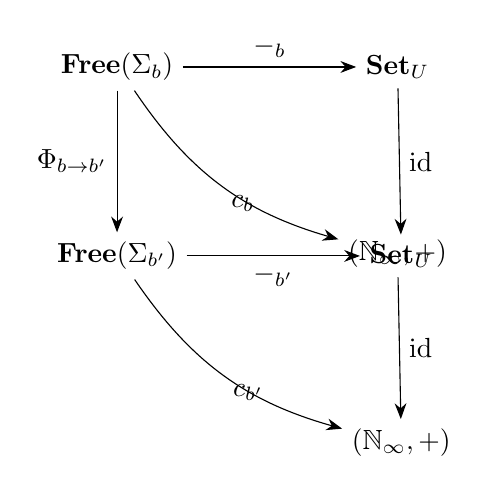
\begin{tikzpicture}[
  node distance = 18mm and 22mm,
  every node/.style = {align=center},
  >={Stealth[length=2mm]}
]
  \node (free) {$\mathbf{Free}(\Sigma_b)$};
  \node[right = of free] (set) {$\mathbf{Set}_U$};
  \node[below = of free] (free2) {$\mathbf{Free}(\Sigma_{b'})$};
  \node[right = of free2] (set2) {$\mathbf{Set}_U$};
  \node[below = of set] (nat) {$(\mathbb{N}_\infty,+)$};
  \node[below = of set2] (nat2) {$(\mathbb{N}_\infty,+)$};

  \draw[->] (free) -- node[above]{$\llbracket - \rrbracket_b$} (set);
  \draw[->] (free2) -- node[below]{$\llbracket - \rrbracket_{b'}$} (set2);
  \draw[->] (free) -- node[left]{$\Phi_{b\to b'}$} (free2);
  \draw[->] (set) -- node[right]{$\mathrm{id}$} (set2);
  \draw[->] (free) to[bend right=20] node[below right]{$c_b$} (nat);
  \draw[->] (free2) to[bend right=20] node[below right]{$c_{b'}$} (nat2);
  \draw[->] (nat) -- node[right]{$\mathrm{id}$} (nat2);
\end{tikzpicture}
\caption{Commutativity of cost and semantics under base shift. Under
the structurality of $c$, both squares commute; the cost-minimal
program shape is therefore preserved by $\Phi_{b\to b'}$.}
\label{fig:diagram}
\end{figure}

\section{Metaphor coherence as a cover}\label{sec:metaphor}

The framework's metaphor labelling provides a categorical refinement.

\begin{definition}[Metaphor cover]
Let $\Pi$ be a finite set of metaphor labels and let $\mu : \Sigma \to
2^\Pi \setminus \{\emptyset\}$ assign to each primitive a non-empty
set of compatible labels. For each $\pi \in \Pi$ let
\[
\Sigma^\pi = \{\sigma \in \Sigma : \pi \in \mu(\sigma)\}
\]
and let $\mathbf{Free}(\Sigma^\pi) \hookrightarrow
\mathbf{Free}(\Sigma)$ denote the full subcategory generated by
$\Sigma^\pi$. The \emph{metaphor cover} is the family
$\{\mathbf{Free}(\Sigma^\pi)\}_{\pi \in \Pi}$.
\end{definition}

\begin{definition}[Metaphor coherence]
A program $P \in \mathbf{Free}(\Sigma)$ is \emph{coherent} if it lies
in some $\mathbf{Free}(\Sigma^\pi)$; equivalently, the metaphor
labels of its constituent primitives have non-empty intersection.
\end{definition}

The set of coherent programs is the union of subcategories
$\bigcup_{\pi \in \Pi} \mathbf{Free}(\Sigma^\pi)$. This is in general
\emph{not} a subcategory of $\mathbf{Free}(\Sigma)$: composing a
program coherent under $\pi$ with one coherent under $\pi' \ne \pi$
may yield an incoherent program. The metaphor cover is therefore a
covering family rather than a single subcategory — closer in spirit to
a Grothendieck topology on $\mathbf{Free}(\Sigma)$ than to a kernel.

\begin{remark}[Sheaf-theoretic interpretation]
A natural extension is to treat $\mu$ as a functor
$\mathbf{Free}(\Sigma) \to \mathbf{Set}$ assigning to each program the
set of metaphors that admit it; coherent programs are those whose
$\mu$-image is non-empty. The semantic functor
$\llbracket - \rrbracket$ then restricts to a section over the
coherent subcategory. Whether useful work can be done at this level
of generality — for example, expressing strategy bridges as
descent data along the cover — is open.
\end{remark}

\section{Synthesis as a fibered problem}

Fix a target function $f \in \mathbf{Set}_U$ and a learner profile
$\ell = (b_w, F, E)$. Restrict to the accessible subcategory
$\mathbf{Free}(\Sigma_E) \subseteq \mathbf{Free}(\Sigma)$ generated by
primitives whose metaphor labels intersect $E$. The
\emph{semantic fibre over $f$ at $\bar{x}$} is
\[
\llbracket - \rrbracket^{-1}\big(f(\bar{x})\big)\big|_{\bar{x}}
\;=\; \big\{ P \in \mathbf{Free}(\Sigma_E) : \llbracket P
\rrbracket(\bar{x}) = f(\bar{x}) \big\}.
\]

\begin{definition}[Productive synthesis]
The \emph{productive program at $(\ell, \bar{x})$} is any element of
\[
\arg\min \Big\{\, c(P, \bar{x}) : P \in \mathbf{Free}(\Sigma_E)
\cap \mathrm{depth}^{-1}([0, b_w])\cap \llbracket -
\rrbracket^{-1}(f(\bar{x})) \,\Big\}.
\]
The argmin is a subset of $\mathbf{Free}(\Sigma_E)$; we write
$P^*(\ell, \bar{x})$ for any chosen representative.
\end{definition}

\begin{definition}[Deformation set]
With $C^* = c(P^*(\ell, \bar{x}), \bar{x})$, the
\emph{cost-bounded deformation set} is
\[
D(\ell, \bar{x}) \;=\; \Big\{\, P \in \mathbf{Free}(\Sigma_E) :
\mathrm{depth}(P) \le b_w,\ c(P, \bar{x}) \le C^*,\ \llbracket P
\rrbracket(\bar{x}) \ne f(\bar{x}),\ P\ \text{coherent}\,\Big\}.
\]
\end{definition}

The deformation set is the union over $\pi \in E$ of the
$\pi$-coherent cost-bounded misses; the metaphor cover restricts the
search exactly as a Grothendieck-topology cover restricts gluing data.

\section{The stratification induced on input space}\label{sec:topology}

For a fixed $(\Sigma, c, \mu, \ell)$ and target $f$ the
\emph{strategy-applicability map}
\[
S_\ell : I \longrightarrow \mathbf{Free}(\Sigma_E)\big/{\cong_{c, \mathrm{depth}}}
\]
sends $\bar{x}$ to the equivalence class of $P^*(\ell, \bar{x})$ under
the relation identifying programs of equal cost and equal depth that
compute the same partial function on the relevant input. The level
sets of $S_\ell$ are a finite partition of $I$ — connected regions on
which a single program (up to the equivalence) is cost-optimal. The
boundaries are loci where two distinct optimal classes meet, i.e.,
where the argmin of $c$ is not a singleton.

We call the collection of level sets, together with the
deformation-set assignment $D(\ell, -)$, the \emph{topology of
arithmetic action} for the given parameters. It is the genuine object
of empirical study once Proposition~\ref{prop:naturality} has reduced
the invariance question to a structurality check on $c$.

\section{Open questions}

\begin{enumerate}[noitemsep,topsep=2pt,label=(\arabic*)]
  \item \textbf{Operadic refinement.} The natural home for the program
        category is a coloured operad. Does the operadic refinement
        improve any of the results above, or does it merely restate
        them? In particular, does the operadic composition give a
        cleaner statement of metaphor-coherence under composition?
  \item \textbf{Cost as enrichment.} The graded cost functor suggests
        $\mathbf{Free}(\Sigma)$ should be enriched over
        $(\mathbb{N}_\infty, +, 0)$, with cost as the hom-set
        valuation. Does this enriched view yield a left Kan extension
        whose value is the productive section, or is the argmin
        irretrievably set-valued?
  \item \textbf{Boundary structure.} The boundaries between strata of
        $S_\ell$ are loci of pedagogical \emph{productive friction}.
        Are these boundaries always of codimension one in $I$? Under
        what conditions on $c$ and $\Sigma$ does the stratification
        carry a Whitney-stratified structure?
  \item \textbf{Descent and strategy bridges.} If the metaphor cover
        is genuinely a Grothendieck topology, descent data along it
        should correspond to documented strategy bridges (e.g.\ the
        rotation-by-$180\degree$ blend that bridges Object Collection
        and Motion-Along-a-Path for integer multiplication). Can
        documented bridges be reconstructed from the descent
        condition?
  \item \textbf{LX as natural transformation.} Brandom's
        LX-relation \parencite{brandom2008meaning} between practices
        is informally diagrammatic: a vocabulary $V'$ stands LX to a
        vocabulary $V$ when $V'$ makes explicit what $V$ admits as
        practice. Does the LX relation lift to a natural
        transformation between the corresponding metaphor
        sub-functors of $\llbracket - \rrbracket$? If so, the cost
        functor's behaviour under LX moves becomes computable from
        the natural-transformation data.
\end{enumerate}

\section*{Note}

This short paper assumes the reader has the longer problem statement
in hand. The cost-bounded synthesis framework, its motivation in the
empirical literature on arithmetic strategies and misconceptions, and
the prototype implementation are all developed there. The point of
the present note is that one of the longer paper's two main claims —
strategic invariance under base shift — is provable on paper under
the structurality condition and does not require empirical
confirmation. What remains computational is the characterisation of
the topology of arithmetic action; what remains philosophically and
formally open is summarised in the questions above.

\printbibliography

\end{document}
